%\VignetteIndexEntry{GAPS/CoGAPS Users Manual}
%\VignettePackage{CoGAPS}

\documentclass{report}
\usepackage{Sweave,fullpage,./chicago,graphicx,subfigure,amssymb,amsmath,color,hyperref,wrapfig}

\author{Elana J. Fertig \\
email: \texttt{ejfertig@jhmi.edu}}
\title{GAPS/CoGAPS Users Manual}

\begin{document}

\maketitle
\tableofcontents

\chapter{Introduction}

\par Gene Association in Pattern Sets (GAPS) infers underlying patterns in a matrix of measurements that can be interpreted as arising from the multiplication of two lower dimensional matrices.  The original development of this R code was focused on gene expression analysis, however the original concept was used in spectral imaging.  The approach is a general form of matrix factorization using a stochastic algorithm.  In this vignette, we will focuson gene expression analysis for concreteness, but the factorization is applicable more broadly.

The Markov chain Monte Carlo (MCMC) matrix factorization that infers patterns also infers the extent to which individual genes belong to these patterns.  The CoGAPS algorithm extends GAPS to infer the coordinated activity in sets of genes for each of the inferred patterns based upon \cite{Ochs2009} and to refine gene set membership based upon \cite{Fertig2012}.

\par The GAPS algorithm is implemented in C++ and compiled and integrated into R using the Rcpp package.  GAPS is licensed under the GNU General Public License version 2.  You may freely modify and redistribute GAPS under certain conditions that are described in the top level source directory file \nolinkurl{COPYING}.

\par The R package CoGAPS is designed to facilitate the corresponding analysis of microarray measurements by calling the GAPS C++ library.  The installation instructions provided in Chapter \ref{install} will insure proper interaction between the CoGAPS R package and GAPS libraries.  Running instructions for the GAPS and CoGAPS analyses are provided in Sections \ref{GAPSRun} and \ref{CoGAPSRun}, respectively.  CoGAPS and GAPS are freely available at \url{https://github.com/ejfertig/CoGAPS} and through the CoGAPS Bioconductor package.  

\par If you use the \texttt{CoGAPS} package for your analysis please cite:
\cite{Fertig2010} EJ Fertig, J Ding, AV Favorov, G Parmigiani, and MF Ochs (2010) CoGAPS: an R/C++ package to identify patterns and biological process activity in transcriptomic data. \textit{Bioinformatics} \textbf{26}: 2792-2793. 

\par To cite the CoGAPS algorithm use:
\cite{Ochs2003} MF Ochs (2003) Bayesian Decomposition in \textit{The Analysis of Gene Expression Data: Methods and Software} G Parmigiani, E Garrett, R Irizarry, and S Zeger, ed. New York: Springer Verlag.

\par To cite the gene set statistic use:
\cite{Ochs2009} MF Ochs, L Rink, C Tarn, S Mburu, T Taguchi, B Eisenberg, and AK Godwin (2009) Detection of treatment-induced changes in signaling pathways in gastrointestinal stromal tumors using transcriptomic data. \textit{Cancer Research} \textbf{69}: 9125-9132.

\par To site the set-membership refinement statistic use:
\cite{Fertig2012} EJ Fertig, AV Favorov, and MF Ochs (2012) Identifying context-specific transcription factor targets from prior knowledge and gene expression data. \textit{2012 IEEE International Conference on Bioinformatics and Biomedicine}, B310, \textit{in press}.

\par Please contact Elana J. Fertig \url{ejfertig@jhmi.edu} or Michael F. Ochs \url{ochsm@tcnj.edu} for assistance. 

\chapter{Installation Instructions} \label{install}

\par The GAPS and CoGAPS algorithms are implemented in an open source C++ software and an R package to facilitate analysis, visualization, and integration with other R tools (CoGAPS, available through Bioconductor).   

\par With this version of CoGAPS, installation should be automatically completed through Bioconductor package loading.


\section{CoGAPS} \label{CoGAPSInstall}

The standard Bioconductor installation for CoGAPS is as follows:
\begin{verbatim}
source("http://www.bioconductor.org/biocLite.R")
biocLite("CoGAPS")
\end{verbatim}


\par Alternatively, the CoGAPS package can be obtained through Bioconductor or Github.  You must first install the boost libraries if you are going to compile on your local machine and then edit the file boostdirs in the \texttt{src} directory to point to your boost include and library file directories.  Next, download the CoGAPS source and install using the following command line argument:
\par \noindent \texttt{R CMD INSTALL CoGAPS}

\par This installation procedure requires administrative privileges to install the CoGAPS package in R.  If you do not have administrative privileges, follow standard R procedures to install the package locally using the lib.loc option in \texttt{install.packages} or \texttt{-l} flag in \texttt{R CMD INSTALL}.

\par In some platforms, the dynamic libraries may not be properly linked for loading the CoGAPS package, leading to an error message such as
\begin{verbatim}
Error in dyn.load(file, DLLpath=DLLpath, ...)  :
  unable to load shared library 'rjags.so'
  libjags.so.1 cannot open shared object file: No such file or directory
Error : .onLoad failed in 'loadNamespace' for 'CoGAPS'
Error: package 'CoGAPS' could not be loaded
\end{verbatim}
In this case, the user should either set the environment variable \texttt{LD\_LIBRARY\_PATH} to \texttt{boostlib\_PATH/lib}.

\subsection{Windows}

\par Installation of CoGAPS on Windows through compiling requires the installation of Rtools and use of the cygwin environment.  Please contact Elana J. Fertig \url{ejfertig@jhmi.edu} or Michael F. Ochs \url{ochsm@tcnj.edu} for installation instructions. 

\chapter{Executing CoGAPS}

\par In this chapter, we describe how to run both the GAPS and CoGAPS algorithms.  

\section{GAPS} \label{GAPSRun}

\par GAPS seeks a pattern matrix (${\bf{P}}$) and the corresponding distribution matrix of weights (${\bf{A}}$) whose product forms a mock data matrix (${\bf{M}}$) that represents the expression data ${\bf{D}}$ within noise limits ($\boldsymbol{\varepsilon}$).  That is,
\begin{equation}
{\bf{D}} = {\bf{M}} + \boldsymbol{\varepsilon} = {\bf{A}}{\bf{P}} + \boldsymbol{\varepsilon}.
\label{eq:matrixDecomp}
\end{equation}
The number of rows in ${\bf{P}}$ (columns in ${\bf{A}}$) defines the number of biological patterns that GAPS will infer from the measured microarray data or equivalently the number of nonorthogonal basis vectors required to span the data space.  As in the Bayesian Decomposition algorithm \cite{Ochs2006}, the matrices ${\bf{A}}$ and ${\bf{P}}$ in GAPS are assumed to have the atomic prior described in \cite{Sibisi1997}.  In the GAPS implementation, $\alpha_{A}$ and $\alpha_{P}$ are corresponding parameters for the expected number of atoms which map to each matrix element in ${\bf{A}}$ and ${\bf{P}}$, respectively.  The corresponding matrices ${\bf{A}}$ and ${\bf{P}}$ are found by MCMC sampling.

\par The GAPS algorithm is run by calling the \texttt{gapsRun} function in the CoGAPS R package as follows:
\begin{verbatim}
> results <- gapsRun(data, unc, nFactor = "5", simulation_id = "simulation", nEquil = "1000", nSample = "1000", nOutR = 1000, output_atomic = "FALSE", alphaA = "0.01",  nMaxA = "100000", max_gibbmass_paraA = "100.0", lambdaA_scale_factor = "1.0", alphaP = "0.01", nMaxP = "100000", max_gibbmass_paraP = "100.0", lambdaP_scale_factor = "1.0")
\end{verbatim}


\par \noindent \textbf{\underline{Input Arguments}}
The inputs that must be set each time are only the data and standard deviation matrices, with all other inputs having default values.  However, in reality it is essential to set at least nFactor, nEquil, and nSample based on the expected dimensionality of the data and the number of iterations needed to explore the posterior distribution.  The arguments are as follows:
\begin{description}
\item[data]{The matrix of m genes by n samples of expression data.  The input should be a matrix object and row names and column names will be retained in the output matrices as appropriate.  }
\item[unc]{The matrix of m genes by n samples of standard deviations for the expression data.  The values will be used in estimating the Likelihood, presently under an assumption of normal error distribution.}
\item[nFactor]{Number of patterns into which the data will be decomposed.  The value must be less than the number of genes and number of samples in the data to avoid instability from an ill-posed problem.}
\item[simulation_id]{The base name to attach to atoms files if created.}
\item[nEquil]{The number of iterations for ``burning in" the sampler before beginning to gather samples for the statistics. The equilibration is done using a simulated annealing approach that slowly lowers the ``temperature" to more thoroughly explore the posterior distribution prior to sampling.}
\item[nSample]{The number of iterations for sampling.  Each iteration refers to a number of proposals chosen from a Poisson distribution with mean equal to the present number of atoms.}
\item[nOutR]{The number of iterations between reporting the present status of the sampler back to R.}
\item[output_atomic]{This determines whether to write atom files to disk (large).}
\item[alphaA]{A sparsity parameter reflecting the expected number of atoms per element of the amplitude $\mathbf{A}$ matrix in the decomposition.  To enforce sparsity, this parameter should typically be less than one. (optional; default=0.01)}
\item[alphaP]{A sparsity parameter reflecting the expected number of atoms per element of the pattern matrix in the decomposition.  To enforce sparsity, this parameter should typically be less than one. (optional; default=0.01)}
\item [max_gibbmass_paraA]{This provides an upper limit on the size of the truncated normal used during Gibbs sampling steps on the A domain.  This avoids the creation of an unusually large mass during sampling when the sampler is in the tail of the truncated normal.}
\item [max_gibbmass_paraP]{This is the corresponding limit for the P domain.}
\item[nMaxA]{This will set a maximum number of atoms in the A domain, however it is not yet implemented in this version.}
\item[nMaxP]{This will set a maximum number of atoms in the P domain, however it is not yet implemented in this version.}
\item[lambdaA_scale_factor]{This is the lambda factor for the penalized likelihood in A.}
\item[lambdaP_scale_factor]{This is the lambda factor for the penalized likelihood in P.}
\end{description}

The algorithm returns in the results a list with
\begin{description}
\item[Amean]{A matrix with the sampled mean value for the amplitude matrix ${{\bf{A}}}$.}
\item[Asd]{A matrix with the sampled standard deviation for the amplitude matrix ${{\bf{A}}}$.}
\item[Pmean]{A matrix with the sampled mean value for the pattern matrix ${\bf{P}}$.}
\item[Psd]{A matrix with the sampled standard deviation for the pattern matrix ${\bf{P}}$.}
\item[atomsAEquil]{A vector with the number of atoms in the A domain throughout the equilibration steps.}
\item[atomsASamp]{A vector with the number of atoms in the A domain throughout the sampling steps.}
\item[atomsPEquil]{A vector with the number of atoms in the P domain throughout the equilibration steps.}
\item[atomsPSamp]{A vector with the number of atoms in the P domain throughout the sampling steps.}
\item[chiSqValues]{A vector with the sample chi-squared values throughput sampling.}
\item[meanChi2]{${\chi^2}$ value of the final mean result, i.e. $\chi^2 = frac{(D-AP)^2{\sigma^2}$.}
\end{description}
  
\par Once the GAPS algorithm has been run, the inferred patterns and corresponding amplitude can be displayed using the \texttt{plotGAPS} function as follows:
\begin{verbatim}
> plotGAPS(Amean, Pmean, outputPDF="")
\end{verbatim}
where setting outputPDF to a string will redirect output to a PDF file from the screen.  The command
\begin{verbatim}
> plotP(Pmean,Psd)
\end{verbatim}
will create a plot of just the rows of the $mathbf{P}$ matrix with standard errors, which is equivalent to plotting the basis vectors for the matrix factorization.

\par \noindent \textbf{\underline{Input Arguments}}
\begin{description}
\item[Amean]{The amplitude matrix ${\bf{Amean}}$ obtained from GAPS.}
\item[Pmean]{The pattern matrix ${\bf{Pmean}}$ obtained from GAPS.}
\item[outputPDF]{Name of an \texttt{pdf} file to which the results will be output.  (Optional; default="" will output plots to the screen.)}
\item[Psd]{The standard deviation of the mean for ${\bf{Pmean}}$.}
\end{description}

\par \noindent \textbf{\underline{Side Effects}}
\begin{itemize}
  \item Save the plots of ${\bf{Amean}}$ and ${\bf{Pmean}}$ to the \texttt{pdf} file \texttt{outputPDF}.
\end{itemize}

\subsection{Examples}

\subsubsection{Simulated data}

\par In this example, we have simulated data in EasySimGS (DGS) with three known patterns (PGS) and corresponding amplitude (AGS) with specified activity in two gene sets (gs).  In this data set, each gene set is overexpressed in of the simulated patterns and underexpressed in one.

<<label=SimCoGAPS,echo=TRUE>>=
library('CoGAPS')
data('EasySimGS')
nIter <- 5e+05 
results <- CoGAPS(data=DGS, unc=0.01, isPercentError=FALSE,
                  GStoGenes=gs,
                  numPatterns=3,
                  SAIter = 2*nIter, iter = nIter,
                  outputDir='GSResults', plot=FALSE)
plotGAPS(results$Amean, results$Pmean, 'GSFigs')
message('Deleting analysis results from CoGAPS for Vignette')
unlink('GSResults', recursive=T)
@

Figure \ref{fig:GS} shows the results from running CoGAPS on the GIST data in \cite{Ochs2009} with the option plot set to true.
\begin{figure}[ht]
\begin{center}
\subfigure[Inferred amplitude matrix]{
\includegraphics[width=0.45\linewidth]{GSFigs_Amplitude}
}
\subfigure[Inferred patterns]{
\includegraphics[width=0.45\linewidth]{GSFigs_Patterns}
}
\end{center}
\caption{Results from GAPS on data of simulated gene set data.}
\label{fig:GS}
\end{figure}

\par Moreover, the gene set activity is provided in \texttt{results\$GSActEst} including p-values for upregulation in \texttt{results\$GSUpreg} and downregulation in \texttt{results\$GSDownreg}.

\subsubsection{GIST data}
\par In this example, we perform the GAPS matrix decomposition on a simulated data set with known underlying patterns (SimpSim) as follows.

<<label=GAPSSimpSim, echo=TRUE>>=
library('CoGAPS')
data('SimpSim')
nIter <- 5000
results <- gapsRun(SimpSim.D, SimpSim.S, nFactor=3,
		nEquil=nIter, nSample=nIter)
plotGAPS(results$Amean, results$Pmean, 'ModSimFigs')
@ 
Figure \ref{fig:ModSim} shows the results from plotting the GAPS estimates of ${\bf{A}}$ and ${\bf{P}}$ using \texttt{plotGAPS}, which has a fit to ${\bf{D}}$ of $\chi^{2}=\Sexpr{results$calcChi2}$.  
\begin{figure}[ht]
  \begin{center}
    \subfigure[Inferred amplitude matrix]{
      \includegraphics[width=0.45\linewidth]{ModSimFigs_Amplitude}
    }
    \subfigure[Inferred patterns]{
      \includegraphics[width=0.45\linewidth]{ModSimFigs_Patterns}
    }
  \end{center}
  \caption{Results from GAPS on simulated data set with known true patterns.}
  \label{fig:ModSim}
\end{figure}
Figure \ref{fig:ModSimPtrue} displays the true patterns used to create the ModSim data, stored in \texttt{SimpSim.P}.
\begin{figure}[ht]
  \begin{center}
<<label=ModSimPtrue, fig=TRUE, echo=FALSE>>=
arrayIdx <- 1:ncol(SimpSim.P)
matplot(arrayIdx, t(SimpSim.P), type='l', lwd=10)
@ 
  \end{center}
  \caption{Known true patterns used to generate ModSim data.}
  \label{fig:ModSimPtrue}
\end{figure}


\section{CoGAPS} \label{CoGAPSRun}

\par CoGAPS infers coordinated activity in gene sets active in each row of the pattern matrix ${\bf{P}}$ found by GAPS.  Specifically, CoGAPS computes a $Z$-score based statistic on each column of the ${\bf{A}}$ matrix developed in \cite{Ochs2009}.  The resulting $Z$-score for pattern $p$ and gene set $i$, $\mathcal{G}_{i}$, with $G$ elements is given by
\begin{equation}
Z_{i,p} = \frac{1}{G} \sum\limits_{g \in \mathcal{G}_{i}} {\frac{{\bf{A}}_{gp}}{{\bf{Asd}}_{gp}}}
\label{eq:avgZ}
\end{equation}
where $g$ indexes the genes in the set and ${\bf{Asd}}_{gp}$ is the standard deviation of ${\bf{A}}_{gp}$ obtained from the MCMC sampling in GAPS.  CoGAPS then uses random sample tests to convert the Z-scores from eq. (\ref{eq:avgZ}) to $p$ values for each gene set.

\par The CoGAPS algorithm is run by calling the \texttt{CoGAPS} function in the CoGAPS R package as follows:
\begin{verbatim}
> results <- CoGAPS(data, unc, GStoGenes, nFactor = "7", nEquil=1000,
                nSample=1000, nOutR=1000, output_atomic="false",
                simulation_id="simulation", plot=TRUE, nPerm=500,
                 alphaA = "0.01",  nMaxA = "100000", 
                 max_gibbmass_paraA = "100.0", lambdaA_scale_factor = "1.0", 
                 alphaP = "0.01", nMaxP = "100000", 
                 max_gibbmass_paraP = "100.0", lambdaP_scale_factor = "1.0") 

\end{verbatim}

\par \noindent \textbf{\underline{Input Arguments}}
\begin{description}
\item[$\ldots$]{Input arguments from GAPS.}
\item[GStoGenes]{List or data frame containing the genes in each gene set. If a list, gene set names are the list names and corresponding elements are the names of genes contained in each set. If a data frame, gene set names are in the first column and corresponding gene names are listed in rows beneath each gene set name.}
\item[nPerm]{Number of permutations used for the null distribution in the gene set statistic. (optional; default=500).}
\item[plot]{Use \texttt{plotGAPS} to plot results from the run of \texttt{GAPS} within \texttt{CoGAPS}.}
\end{description}
  
\par \noindent \textbf{\underline{List Items in Function Output}}
\begin{description}
\item[$\ldots$]{Output list from GAPS except vectors of sample atom numbers and individual $\chi^2$ values.}
\item[D]{The input data matrix.}
\item[Sigma]{The input standard deviation matrix.}
\item[GSUpreg]{p-values for upregulation of each gene set in each pattern.}
\item[GSDownreg]{p-values for downregulation of each gene set in each pattern.}
\item[GSActEst]{Conversion of p-values to activity estimates of each gene set in each pattern (see \cite{Ochs2009} for details on conversion.  Essentially values near $1$ indicate high activity for the set and near $-1$ indicate low activity.}
\end{description}

\par The CoGAPS algorithm can also be run manually by first running the GAPS algorithm described in Section \ref{GAPSRun} and then calling the function \texttt{calcCoGAPSStat} as follows:
\begin{verbatim}
> calcCoGAPSStat(Amean, Asd, GStoGenes, numPerm=500)
\end{verbatim}
The input arguments for \texttt{calcCoGAPSStat} are as described in the previous sections.  This function will output a list containing \texttt{GSUpreg}, \texttt{GSDownreg}, and \texttt{GSActEst}.

\subsubsection{Simulated data}

\par In this example, we have simulated data in EasySimGS (DGS) with three known patterns (PGS) and corresponding amplitude (AGS) with specified activity in two gene sets (gs).  In this data set, each gene set is overexpressed in of the simulated patterns and underexpressed in one.

<<label=SimCoGAPS,echo=TRUE>>=
library('CoGAPS')
data('SimpSim')
nIter <- 5000 
results <- CoGAPS(D, S, GSets,
                  numPatterns=3,
                  nEquil=nIter, nSample=nIter
                  plot=FALSE)
plotGAPS(results$Amean, results$Pmean, 'GSFigs')
message('Deleting analysis results from CoGAPS for Vignette')
unlink('GSResults', recursive=T)
@

Figure \ref{fig:GS} shows the results from running CoGAPS on the GIST data in \cite{Ochs2009} with the option plot set to true.
\begin{figure}[ht]
\begin{center}
\subfigure[Inferred amplitude matrix]{
\includegraphics[width=0.45\linewidth]{GSFigs_Amplitude}
}
\subfigure[Inferred patterns]{
\includegraphics[width=0.45\linewidth]{GSFigs_Patterns}
}
\end{center}
\caption{Results from GAPS on data of simulated gene set data.}
\label{fig:GS}
\end{figure}

\par Moreover, the gene set activity is provided in \texttt{results\$GSActEst} including p-values for upregulation in \texttt{results\$GSUpreg} and downregulation in \texttt{results\$GSDownreg}.

\subsubsection{GIST data}

\par We also provide the code that repeats the CoGAPS analysis of GIST data (GIST\_TS\_20084) with gene sets defined by transcription factors (TFGSList), as in the DESIDE analysis of \cite{Ochs2009}.  To minimize time in running the vignette, this is not done live.  However, running the code will complete the analysis and require on the order of an hour on a fast machine.

<<keep.source=T, eval=FALSE>>=
library('CoGAPS')
data('GIST_TS_20084')
data('TFGSList')
nIter <- 10000 
results <- CoGAPS(GIST.D, GIST.S, tf2ugFC,
                  nFactor=5,
                  nEquil=nIter, nSample=nIter,
                  plot=FALSE)
plotGAPS(results$Amean, results$Pmean, 'GISTFigs')
# message('Deleting analysis results from CoGAPS for Vignette')
# unlink('GISTResults', recursive=T)
@  

Figure \ref{fig:GS} shows the results from running CoGAPS on the GIST data in \cite{Ochs2009} with the option plot set to true.
\begin{figure}[ht]
\begin{center}
\subfigure[Inferred amplitude matrix]{
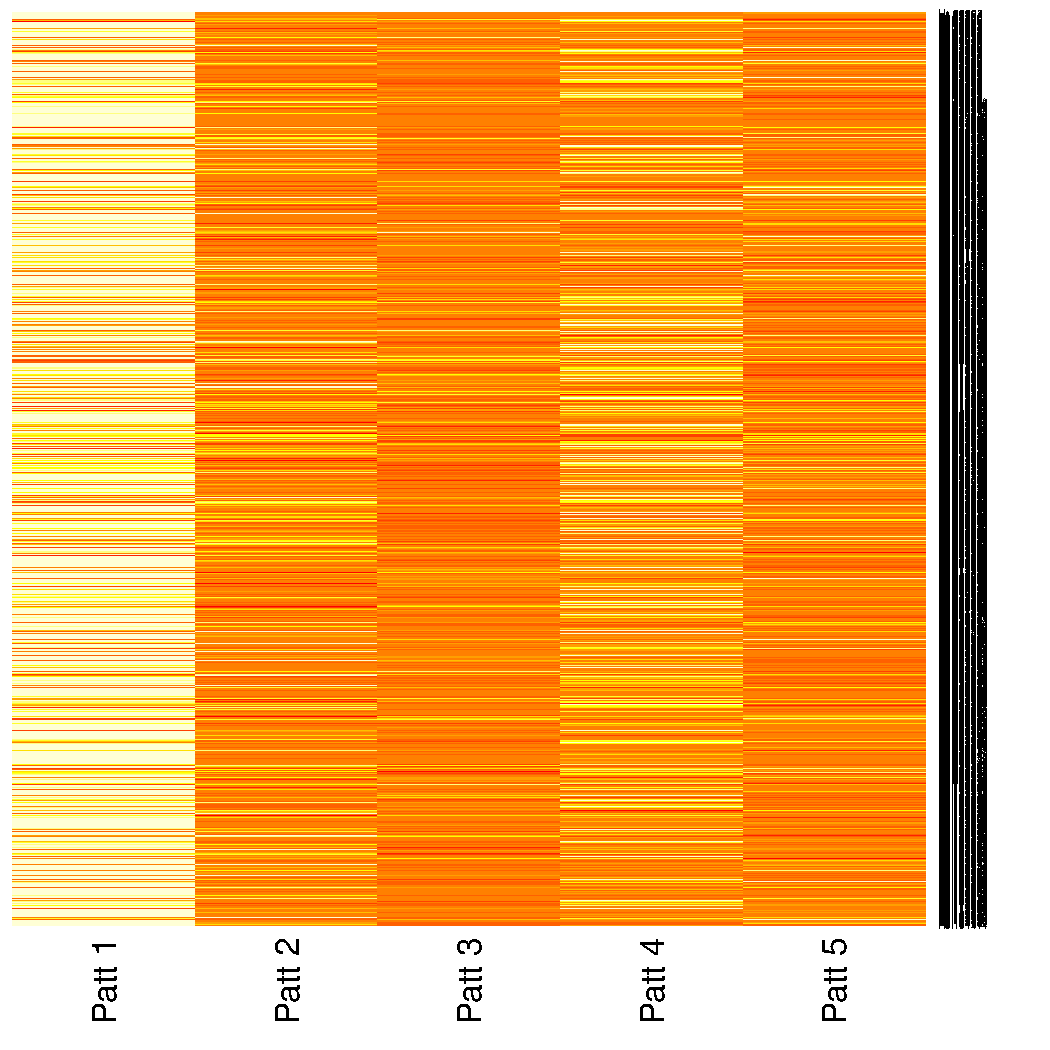
\includegraphics[width=0.45\linewidth]{GISTFigs_Amplitude}
}
\subfigure[Inferred patterns]{
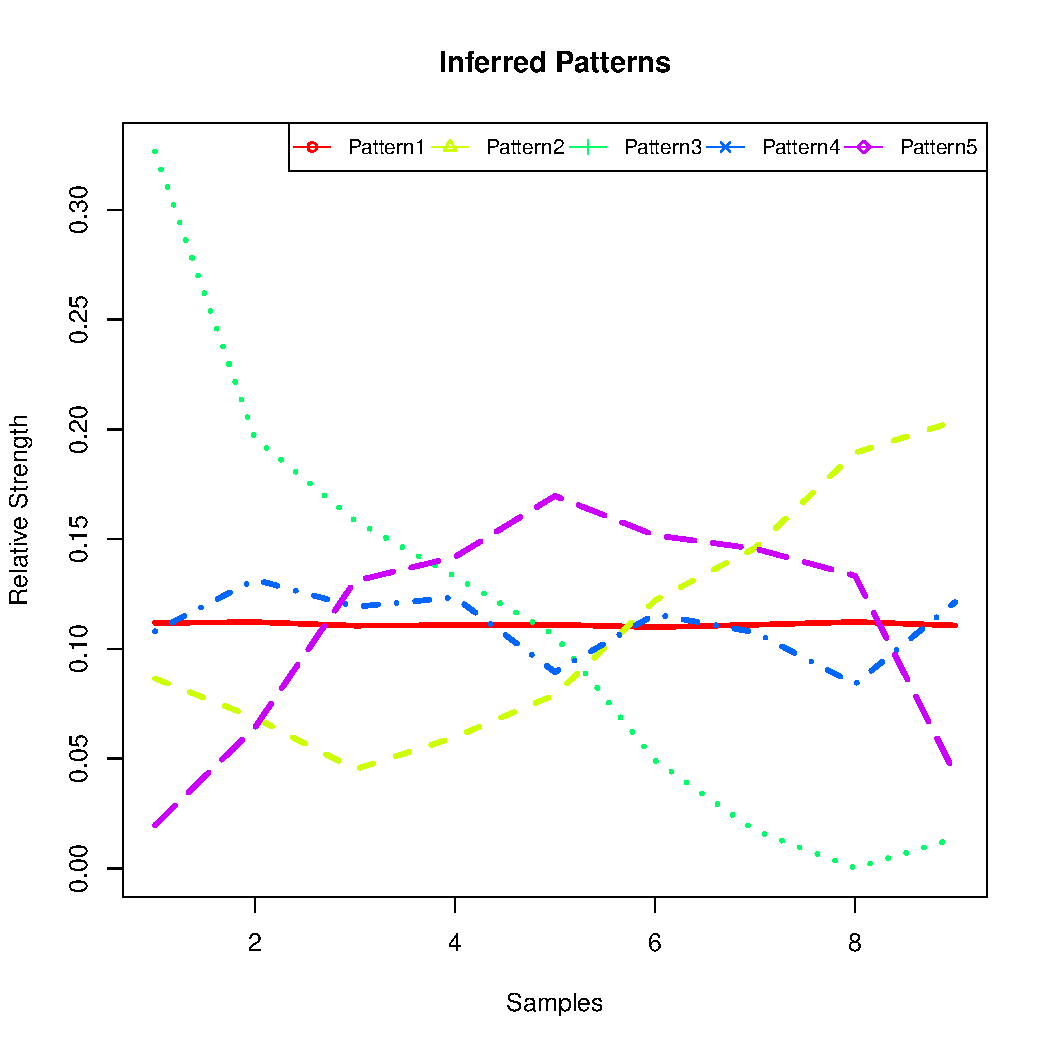
\includegraphics[width=0.45\linewidth]{GISTFigs_Patterns}
}
\end{center}
\caption{Results from GAPS on data of simulated gene set data.}
\label{fig:GS}
\end{figure}

\par Moreover, the gene set activity is provided in \texttt{results\$GSActEst} including p-values for upregulation in \texttt{results\$GSUpreg} and downregulation in \texttt{results\$GSDownreg}.

\section{Using CoGAPS-based statistics to infer gene membership in annotated gene sets}

\par As we describe in the previous section, the GAPS matrix factorization can be used to infer gene set activity in each pattern using the function \texttt{calcCoGAPSStat} \cite{Ochs2009}.  The \texttt{computeGeneGSProb} function extends this gene set statistic to compute a statistic quantifying the likely membership of each gene annotated to a set based upon its inferred activity \cite{Fertig2012}.  This statistic is formulated by comparing the expression pattern computed with CoGAPS of a given gene $g$ annotated as a member of $\mathcal{G}$ to the common expression pattern of all annotated members of $\mathcal{G}$.  This similarity is quantified with the following summary statistic
\begin{equation}
S_{g,\mathcal{G}} = \frac{\sum_{p} -log\left(\mbox{Pr}_{\mathcal{G}p}\right){\bf{A}}_{gp}/{\bf{Asd}}_{gp}}{\sum_{p} -log\left(\mbox{Pr}_{\mathcal{G}p}\right)},
\label{eq:summaryGSStat}
\end{equation}
where $\mbox{Pr}_{\mathcal{G}p}$ is the probability of upregulation of the geneset, returned from \texttt{calcCoGAPSStat} as \texttt{GSActEst} based upon eq.~(\ref{eq:avgZ}).  Similar to the gene set statistics, p-values for the set membership are computed with permutation tests that compare the value of $S_{g,\mathcal{G}}$ from eq.~(\ref{eq:summaryGSStat}) to the statistic formulated for a random gene set of the same size that also contains gene $g$.  

\par The set membership statistic is computed from the results from the GAPS matrix factorization, computed with either the \texttt{GAPS} function described in Section \ref{GAPSR un} or the \texttt{CoGAPS} function described in Section \ref{CoGAPSRun} as follows:
\begin{verbatim}
> computeGeneGSProb(Amean, Asd, GStoGenes, numPerm=500)
\end{verbatim}

\par \noindent \textbf{\underline{Input Arguments}}
\begin{description}
\item[Amean]{Mean of the amplitude matrix estimated from the GAPS matrix factorization}
\item[Asd]{Standard deviation of the amplitude matrix estimated from the GAPS matrix factorization}
\item[GStoGenes]{List or data frame containing the genes in each gene set. If a list, gene set names are the list names and corresponding elements are the names of genes contained in each set. If a data frame, gene set names are in the first column and corresponding gene names are listed in rows beneath each gene set name.}
\item[nPerm]{Number of permutations used for the null distribution in the gene set and set membership statistics. (optional; default=500).}
\end{description}
  
\par \noindent \textbf{\underline{Function Output}}
\begin{description}
\item p-value of set membership for each gene specified in \texttt{GStoGenes}.
\end{description}

\subsection{Example on GIST Data}

\par Although not run in the interest of installation time, the following examples were used to generate some of the results in \cite{Fertig2012}, with the complete analysis code available from \url{http://astor.som.jhmi.edu/~ejfertig/ejfertig/Publications.html}.

\par This example refines transcription factor targets annotated in TRANSFAC (TFGSList) to identify context-specific targets from gene expression data (GIST\_TS\_20084)from \cite{Ochs2009}.  

<<eval=FALSE, keep.source=TRUE>>=

# define transcription factors of interest based on Ochs et al. (2009)
TFs <- c("c.Jun", 'NF.kappaB', 'Smad4', "STAT3", "Elk.1", "c.Myc", "E2F.1",
         "AP.1", "CREB", "FOXO", "p53", "Sp1")

# take the results from the previously run analysis
# set membership statistics
permTFStats <- list()
for (tf in TFs) {
     genes <- levels(tf2ugFC[,tf])
     genes <- genes[2:length(genes)]
     permTFStats[[tf]] <- computeGeneTFProb(Amean = results$Amean,
                                            Asd = results$Asd, genes)
}
@

\chapter{Feedback}

\par Please send feedback to Elana Fertig \texttt{ejfertig@jhmi.edu} or Michael Ochs \texttt{ochsm@tcnj.edu}.

\par If you want to send a bug report, please first try to reproduce the error.  The code is stochastic and we have seen many transient errors arising in the boost libraries which rarely repeat.  Send the data and please describe what you think should have happened, and what did happen.

\chapter{Acknowledgments}

\par Special thanks to paper co-authors Jie Ding, Alexander V. Favorov, and Giovanni Parmigiani for statistical advice in developing the GAPS / CoGAPS algorithms.  Additional thanks to Simina M. Boca, Ludmila V. Danilova, Jeffrey Leek, and Svitlana Tyekcheva for their useful feedback.

\par This work was funded by NIH/NLM R21LM009382, NIH/NLM R01LM011000 and NSF Grant 0342111. 

\bibliographystyle{plain}
\bibliography{AppNote}

\end{document}
